 \documentclass[conference]{IEEEtran}
\IEEEoverridecommandlockouts
% The preceding line is only needed to identify funding in the first footnote. If that is unneeded, please comment it out.
\usepackage{cite}
\usepackage{cite}
\usepackage{amsmath,amssymb,amsfonts}
\usepackage{algorithmic}
\usepackage{textcomp}
\usepackage{xcolor}
\def\BibTeX{{\rm B\kern-.05em{\sc i\kern-.025em b}\kern-.08em
    T\kern-.1667em\lower.7ex\hbox{E}\kern-.125emX}}
    
    
\usepackage{epsfig}
\usepackage{amsmath}
\usepackage{graphicx}% Include figure files
\usepackage{dcolumn}% Align table columns on decimal point
\usepackage{bm}% bold math
\usepackage{amssymb}
\usepackage{amsmath}
\usepackage{epsf}
\usepackage{subfigure}
\usepackage{epstopdf}
\usepackage{color}
\usepackage{subeqnarray}
\usepackage{mathrsfs}
\usepackage{array}
\usepackage{tabularx}
\usepackage{placeins}


\usepackage[colorlinks=true, pdfstartview=FitV, linkcolor=red, citecolor=blue, urlcolor=blue]{hyperref}
\usepackage{amsmath,amssymb,amsfonts}
\usepackage{algorithmic}
\usepackage{graphicx}
\usepackage{textcomp}
\usepackage{xcolor}
\def\BibTeX{{\rm B\kern-.05em{\sc i\kern-.025em b}\kern-.08em
    T\kern-.1667em\lower.7ex\hbox{E}\kern-.125emX}}
\begin{document}

\title{Opportunistic Spinlock\\
\thanks{Identify applicable funding agency here. If none, delete this.}
}

\author{\IEEEauthorblockN{1\textsuperscript{st} Jay Shah}
\IEEEauthorblockA{\textit{ICT Student} \\
\textit{DAIICT}\\
Gandhinagar, India \\
201801141@daiict.ac.in}
\and
\IEEEauthorblockN{2\textsuperscript{nd} Shubham Makwana  }
\IEEEauthorblockA{\textit{ICT Student} \\
\textit{DAIICT}\\
Gandhinagar, India \\
201801213@daiict.ac.in}
}

\maketitle

\begin{abstract}
With increasing demand for big-data processing and faster in-memory
databases, cloud providers are moving towards large virtualized instances
besides focusing on the horizontal scalability.
However, experiments reveal that such instances in popular cloud services
(e.g., 32 vCPUs with 208 GB supported by Google Compute Engine) do not
achieve the desired scalability because of the sophisticated optimization
techniques implemented in the hypervisor—what is called as sleepy spinlock
anomaly. Opportunistic spinlock tries to address this sleepy spinlock anomaly.
\newline
\end{abstract}

\section{Introduction}
To solve this problem, this paper presents the design and implementation of OTICKET (Opportunistic spinlock), a variant of paravirtualized ticket spinlock that effectively scales the virtualized instances.

\subsection{LHP and LWP problem in virtualized environment
}\label{AA}

\begin{itemize}
\item Assumption in traditional Spinlock implementation 
  \begin{itemize}
    \item Lock holder thread and lock waiter threads can not be preempted
  \end{itemize}
\item vCPU can be preempted by hypervisor
\item Lock Holder Preemption problem(LHP) occurs when vCPU that is holding the
lock gets preempted and none of the waiter thread can make the progress.

\item Lock Waiter Preemption problem(LWP) occurs because of the FIFO
implementation for waiter threads. None of the threads can make the
progress unless the exact next waiter is scheduled.
\item  Paravirtual spinlock addresses this problem
\newline
\end{itemize}

\section{Paravirtual spinlock}
\begin{itemize}
\item Two routines for lock waiter threads
  \begin{itemize}
    \item 1. Fast path \space 2. slow path
  \end{itemize}
\item Fast path routine: Lock waiter thread spins for some fixed number of iteration
if it fails to acquire the lock it falls back to slow path
\item Slow path routine: Lock waiter thread issues a halt instruction which gets
trapped by the hypervisor. Hypervisor schedules out the waiter and voluntary
yields to the other vCPU
\item Unlock phase: During the unlock phase holding vCPU wakes up the next
waiter via kick hyper call and precisely wakes up the next vCPU.
\item This lock solves both the problem LHP and LWP.
\newline
\end{itemize}

\section{Performance Issue in Paravirtual Spin lock}
Theoretically the performance of PV spin
lock should be better, but surprisingly as
the count of vCPU increases from 20 to
30 there a sudden collapse in
performance. This is due to the increasing number of
halt instruction after 30 vCPU since most
of the vCPU will fail to acquire the lock in
fast path.
This issue is called as sleepy spin lock
anomaly
\newline

%add the image .......
\begin{figure}
        \centering
       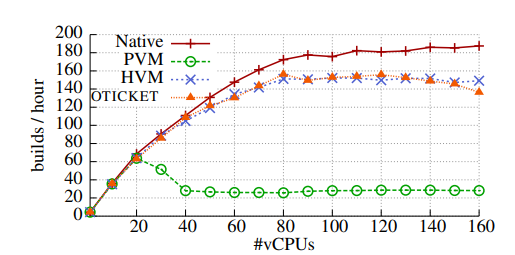
\includegraphics[scale=0.9]{Performance_1.PNG}~
       \caption{ Performance of a Linux kernel compile on an 80-core machine.We enabled hyperthreads per core, }\label{Fig:1}
 \end{figure}

\section{Opportunistic ticket spin lock (OTICKET)}
This article proposes opportunistic spin lock which is improvement on
paravirtualized spin lock.
It improves the sleepy spin lock anomaly and addresses the LHP and LWP
problem.
Similar to paravirtual spin lock OTICKET is composed of two paths namely
fast path and slow path in locking routine.
Lock waiter first spins in the fast path and then falls back to the slow path if it
does not able to acquire the lock.
In addition to that there two schemes opportunistic spinning
and opportunistic wake up.

\subsection{Optimal decision on spinning and waking up in OTICKET}
In order to make the optimal decision on spinning and waking up OTICKET
uses the distance between the lock holder thread and lock waiter thread into
consideration.
 Since in FIFO ordering of waiters, it assumes that time required to acquire the
lock is almost proportional to the waiter’s distance.
Both the scheme helps to improve the sleepy spin lock anomaly by keeping
the waiters which are nearer to lock holder into fast path, thereby decreasing
the halt instructions.
\subsection{Opportunistic spinning}
 In the opportunistic spinning the closer waiters opportunistically spin for
longer duration in fast path, hoping to get the lock sooner.
If the lock is acquired while spinning the vCPU can avoid the costly switching
between the guest os and hypervisor in halt instruction.
 And as the distance of lock waiter increases the spinning iteration
exponentially decreases.

\subsection{Opportunistic wakeup}
Waking up the halter CPU takes the significant time, since it involves notifying
the hypervisor.
In order to avoid this time, at the time of unlocking OTICKET allows the lock
holder to wake up the next N waiters in advance.
So that they will get back to the fast path and will start spin for the lock.
\newline

\section{Implementation}
\subsection{Modifying the code}
\begin{figure}[!h]
    \centering
    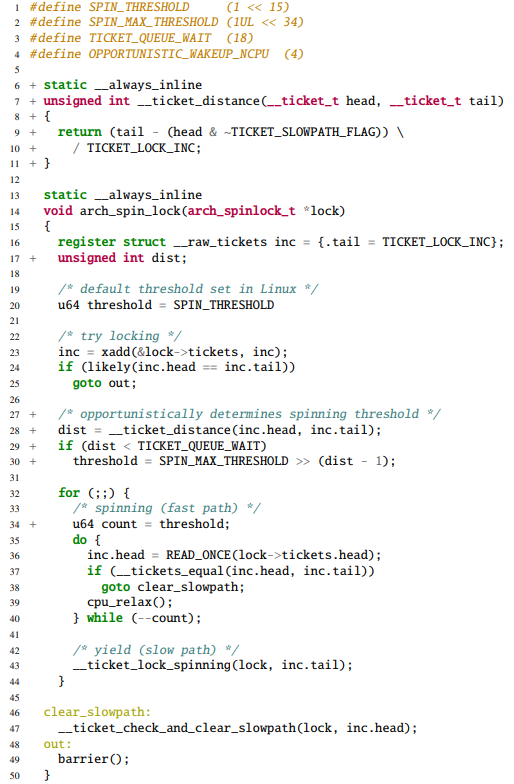
\includegraphics[scale = 0.88]{Implementation_1.png}
    \caption{Distance and locking function}
    \label{Fig.2}
\end{figure}
\FloatBarrier

\begin{figure}[!h]
    \centering
    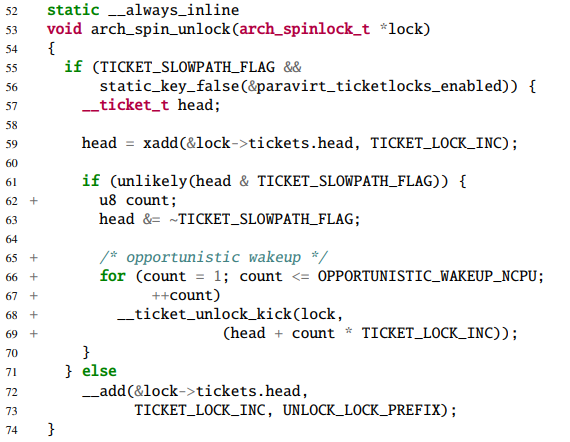
\includegraphics[scale = 1.0]{Implementation_2.PNG}
    \caption{Unlock function}
    \label{Fig.3}
\end{figure}
\FloatBarrier

\subsection{Kernel Compilation with Linux kernel version 4.4.274}
  \begin{itemize}
    \item Steps followed:
  \end{itemize}
\begin{enumerate}
\item tar xvf linux-4.4.274.tar.xz (Unzip folder)
\item sudo apt-get install git fakeroot build-essential ncurses-dev xz-utils libssl-dev
bc flex libelf-dev bison (Install essential packages)
\item cd linux-4.4.274
\item cp -v /boot/config-\$(uname -r) .config (copy existing configuration file)
\item make menuconfig
a) general setup
b) enabled Automatically append version information to the version string
\item make // building kernel
\item sudo make modules\textunderscore install (install required modules)
\item sudo make install
\item GRUB bootloader is the first program that runs when system powers on.
Changed GRUB file so that new kernel boots.
\item uname -mrs (to verify the kernel version)
\end{enumerate}


\section{Performance Evaluation}
\begin{figure}[!h]
    \centering
    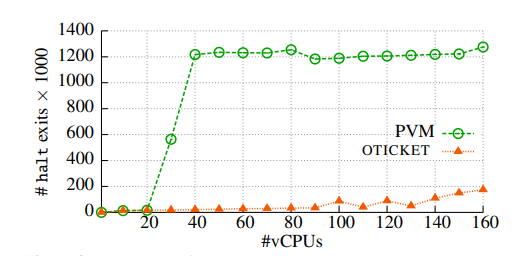
\includegraphics[scale = 1.0]{Performance_2.PNG}
    \caption{Number of halt instructions in PVM vs OTICKET}
    \label{Fig.3}
\end{figure}
\FloatBarrier
As above figure shows the number of halt instruction in Paravirtual spin lock increases as the number of vCPU increases. Where as it remains constant for Opportunistic spin lock.
It reveals that the voluntary sleeping optimization
for the virtualized environments can result in performance collapse
(sleepy spin lock anomaly) for the kernel-intensive workloads, which opportunistic spin lock tries to avoid.
\newline

\section{Conclusion}
This paper analyze the scalability performance of a VM on an 80-core machine for the Linux kernel compilation benchmark.
The use of spinlock, which guarantees strict FIFO ordering, is another culprit for the performance degradation.
The paper provide a variant of the ticket spinlock implementation to address this problem and resolve this issue for VMs with large vCPU count.
\newline

\section{GitHub Repository}
\url{https://github.com/JayShah610/Opportunistic\textunderscore spinlocks}
\newline


\begin{thebibliography}{00}
\bibitem{b1} Kashyap, Sanidhya et al. “Opportunistic Spinlocks: Achieving Virtual Machine Scalability in the Clouds.” ACM SIGOPS Oper. Syst. Rev. 50 (2016): 9-16.

\end{thebibliography}
\vspace{12pt}

\end{document}
